\section{Complete grid results}\label{app:minimal-grid}
All 480 fits complete without nonfinite updates. Recovery and query-count
checks pass in all 80 paired cache conditions. Maximum coefficient
error is $2.49\times10^{-15}$; relevant/full normalized-regret difference
is at most $3.81\times10^{-12}$, meeting the tolerance in all 80 pairs.
Maximum parameter difference is $8.94\times10^{-7}$. Re-evaluation
reproduces every scalar metric; telescoping error is at most
$7.74\times10^{-14}$.

Box caches require 332,362 relevant responses versus 1,039,456 for
full-face recovery, a 68.03\% reduction. At $d=32,m=2,R=0.5$ the
reduction is 85.20\%, or 0.995 versus 6.722 queries per state including
inactive targets. Table~\ref{tab:minimal-feedback} gives all box conditions.
\begin{table}[htbp]
\centering\small
\caption{Scalar feedback in the box experiment. Queries are means per cached state, including interior targets. Savings compare relevant queries with full normal-space reconstruction. Coefficient errors are relative RMS errors averaged over five seeds; these are information diagnostics, not policy costs.}\label{tab:minimal-feedback}
\begin{tabular}{lrrrrr}\toprule
$d,m,R$ & Relevant & Full face & Saved (\%) & Gain error & Random error\\\midrule
8,2,0.5 & 0.876 & 1.592 & 45.0 & 0.108 & 0.184\\
8,2,2 & 0.073 & 0.073 & 0.0 & 0.000 & 0.000\\
8,4,0.5 & 1.388 & 1.592 & 12.8 & 0.107 & 0.107\\
8,4,2 & 0.073 & 0.073 & 0.0 & 0.000 & 0.000\\
32,2,0.5 & 0.995 & 6.722 & 85.2 & 0.194 & 0.379\\
32,2,2 & 0.072 & 0.072 & 0.0 & 0.000 & 0.000\\
32,4,0.5 & 1.861 & 6.722 & 72.3 & 0.178 & 0.326\\
32,4,2 & 0.072 & 0.072 & 0.0 & 0.000 & 0.000\\
\bottomrule\end{tabular}
\end{table}

\begin{figure}[htbp]\centering
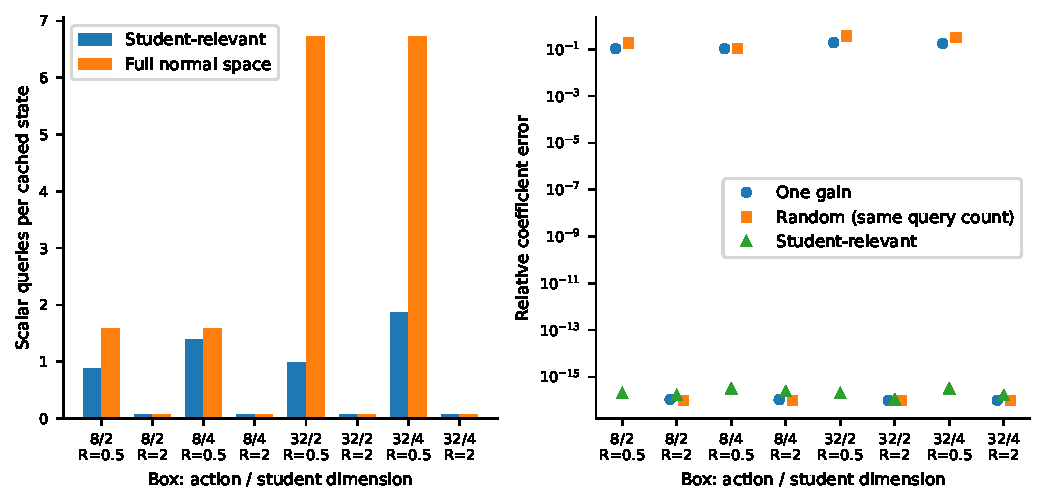
\includegraphics[width=\linewidth]{figures/minimal_information.pdf}
\caption{Box query counts and relative coefficient errors, averaged over
five seeds. Relevant and random methods use the same number of responses;
gain uses one per active target.}\label{fig:minimal-information}
\end{figure}

On balls, all four scalar recovery methods reproduce full-information
learning. Sampled boxes at $R=2$ have at most one active coordinate,
so gain and random also recover exactly and no query saving occurs.
At $R=0.5$, their condition-mean coefficient errors range from 0.107
to 0.379. Policy effects are smaller: for $d=32,m=2,R=0.5$, relevant,
gain and random regrets are 0.90062, 0.90285 and 0.90632.

Relevant feedback lowers mean regret and cost versus target-only in all
16 conditions. For each endpoint, three unadjusted intervals include
zero: both eight-dimensional ball conditions with $m=4$, and the
eight-dimensional box with $m=4,R=2$ (\ref{app:minimal-comparisons}).
High remaining regret in small subspaces reflects limited representability.

Algebraic checks cover 576 recovery cases through dimension 128,
including a nonzero student-orthogonal normal needing no query.
Another 120 constructions use $r-1$ queries: admissible normals yield
identical responses within $6.40\times10^{-17}$ but different student
coefficients. They also verify Eq.~\eqref{eq:minimal-noise} for response
error norms up to $10^{-3}$. These checks involve no additional training.
